\documentclass{article}


\usepackage{PRIMEarxiv}

\usepackage[utf8]{inputenc}
\usepackage[T1]{fontenc}
\usepackage{natbib}
\usepackage{hyperref}
\usepackage{url}
\usepackage{booktabs}
\usepackage{amsmath}
\usepackage{amsfonts}
\usepackage{nicefrac}
\usepackage{microtype}
\usepackage{fancyhdr}
\usepackage{graphicx}
\graphicspath{{figures/}}
\usepackage{caption}
\usepackage{subcaption}
\usepackage[table]{xcolor}
\usepackage{array}

% NOTATION 
\newcommand{\R}{\mathbb R}

\renewcommand{\t}{\theta}

\pagestyle{fancy}
\thispagestyle{empty}
\rhead{ \textit{ }} 

% UPDATE HEADERS
\fancyhead[LO]{}
% \fancyhead[RE]{Firstauthor and Secondauthor} % Firstauthor et al. if more than 2 - must use \documentclass[twoside]{article}

%% UPDATE TITLE
\title{ProtoTSRL: Interpretable Time Series Representation Learning}
\author{
    Haiyan Wang \\
    Duke University \\
    \texttt{haiyan.wang916@duke.edu}
}

\begin{document}
\maketitle

\begin{abstract}
\end{abstract}

% UPDATE KEYWORDS
% \keywords{First keyword \and Second keyword \and More}

% %%%%%%%%% INTRODUCTION %%%%%%%%%

\section{Introduction}
\label{sec:intro}

Time series are prevalent across a wide range of domains and often drive decisionmaking in high-stakes environments including health monitoring, weather forecasting, and financial modeling. However, time series data pose significant challenges for human interpretability due to their high dimensionality with respect to both the length of the series and the number of features in each observation. Moreover, real-world time series data often present with irregularities such as temporal misalignment, uneven lengths, and variable sampling frequencies which can further obfuscate important structure. As a result, time series data are often sparsely labeled, and it is infeasible to annotate large datasets to the extent required for supervised modeling. The ability to learn fixed-length representations of time series without explicit supervision that differentiate relevant patterns from nuisance variation is important for both identifying latent structure within time series data as well as for downstream tasks such as classification and forecasting. 

In this paper, we propose ProtoTSRL, a new approach to learning informative, general-purpose representations of time series that is both \textit{interpretable} and \textit{domain-agnostic}. Our primary contributions are: 
\begin{itemize}
    \item A contrastive learning framework that incorporates insights from dimension reduction algorithms by introducing a third class of contrasting samples separate from positive and negative pairings. Unlike previous approaches, contrastive samples are created with both sampling- and augmentation-based methods and do not rely on domain-specific assumptions such as local smoothness.
    \item A novel architecture that employs multiscale prototype-based learning to capture both local morphological traits and global temporal dynamics. The proposed architecture can be trained in stages, allowing us to shape semantic intermediate latent spaces which are then used to learn final representations.
\end{itemize}

% %%%%%%%%% RELATED WORK %%%%%%%%%

\section{Related Work}
\label{sec:rw}

In the most general sense, representation learning refers to techniques that learn to extract and represent useful information from raw data. This is evidently a broad definition and many methods and models fall under this umbrella including clustering, dimension reduction, and neural networks. Here, we review methods for learning representations without explicit supervision, and in particular, on self-supervised methods. Prior work indicates that learning to solve appropriately designed auxiliary tasks based on data-derived pseudolabels induces models to represent important semantic information embedded in unlabeled data \cite{bengio13-rlsurvey, jing21-visualrl, mohamed22-speechrl}. This is of particular importance for time series data which frequently lack human-recognizable attributes but yield well to pseudolabeling.

A common auxiliary task is learning to reverse augmentations. This is a particularly popular approach for visual data and computer vision (CV) -- augmentations include decolorization \cite{zhang16-colorization}, masking \cite{pathak16-inpainting}, and scrambling \cite{noroozi17-puzzle}. In this case, the original image or some subpart of it is used as the pseudolabel to guide learning, and such approaches assume that data may be characterized by semantic information that is invariant under augmentation. Other auxiliary tasks are contrastive (e.g. \cite{vandenoord19-cpc, tian20-cmc}) -- rather than learning to extract information that characterizes samples, these models learn to extract information that differentiates samples. When applied to downstream tasks such as classification, object detection, and segmentation, the learned representations match or outperform fully supervised training from scratch \cite{jing21-visualrl}. Representation learning has also been successful in settings that involve sequential data. In natural language processing (NLP), algorithms like Word2Vec \cite{mikolov13-word2vec} learn static embeddings for words based on the contexts in which each word was found throughout a large training corpus. Subsequent developments such as Doc2Vec \cite{le14-doc2vec} learned fixed-length representations of entire variable-length passages. Such representations are applied in downstream tasks like topic modeling \cite{angelov20-top2vec} and machine translation \cite{sutskever14-seq2seq}. The invention of the transformer architecture \cite{vaswani17-transformer} further advanced the ability to generate contextual representations via models like BERT \cite{devlin19-bert}. The auxiliary tasks learned by these models are simple predictive problems such as masked- or next- token prediction. Similar techniques (e.g. \cite{vandenoord17-vqvae, chung20-apc, baevski20-wav2vec}) are applied to tasks involving audio data despite its higher complexity relative to language: it is significantly higher dimensional, continuous, and contains many entangled components that don't yield well to segmentation \cite{mohamed22-speechrl}. 

The success of representation learning across such a wide range of data modalities suggests it may be well-suited for application to time series data. Broadly speaking, there are two types of representations that can be learned for a multivariate time series: instance-level representations capture entire series, encompassing multivariate observations across multiple timestamps, while semantic-level representations capture each timestamp individually. The primary focus of existing literature is designing appropriate auxiliary tasks. Some of these tasks are borrowed directly from other fields: for example, drawing inspiration from BERT, encoder-only transformers have learned effective representations by reconstructing masked observations or subsegments within a longer time series \cite{zerveas21-tsbert}. SOM-VAE \cite{fortuin19-somvae} learns representations at a semantic level and opts for a reconstructive auxiliary task: a variational autoencoder (VAE) learns a semantic latent space that is shaped by a discrete self-organizing map (SOM). Given a multivariate time series, the observation at each timestamp is mapped to a continuous latent vector which is then assigned to its nearest SOM embedding. The decoder reconstructs the observation from both the continuous embedding and its SOM label. To represent temporal dynamics, a Markov transition model is learned over the discrete SOM states to predict the state of the next observation in the series. 

Other prior methods implement contrastive auxiliary objectives, raising the question of how best to define contrastive examples. Two major approaches are reflected in the literature: sampling and augmentation. Sampling is usually time-based (e.g. \cite{franceschi19-timesampling}) and draws inspiration from previous successes in NLP. Time-based sampling assumes that, given an arbitrary subseries sampled from a larger time series, temporally close subseries should have similar representations while distant subseries (temporally distant in the same series or from another series) should have different representations. An obvious weakness of time-based sampling is the strong assumption of local smoothness which may not hold for series with sudden distribution changes. TNC \cite{tonekaboni21-tnc} addresses this with a weaker assumption of local smoothness by drawing positive examples for a given subseries from a normal distribution centered at that subseries, the variance of which is a tunable hyperparameter. Additionally, TNC employs positive-unlabeled learning, a variant of contrastive learning which treats nonpositive samples as unknown and reweights their contribution to the overall contrastive loss. The other approach to defining contrastive examples is via augmentation. TS-TCC \cite{eldele21-tstcc} creates different views of the same series with weak (scaling and jittering) and strong (permutation and jittering) augmentations. These views are encoded to an intermediate latent space shaped by a temporal contrasting objective based on cross-view prediction. Intermediate embeddings are then mapped by a nonlinear function to the final representation space which is shaped by a standard contrasting objective. This framework encourages the model to learn both temporal and discriminative patterns that are preserved under augmentation. Lastly, TS2Vec \cite{yue21-ts2vec} also learns semantic-level representations, but these representations can be aggregated into instance-level representations. TS2Vec defines positive pairs by sampling overlapping subseries which are randomly masked and cropped to form distinct contexts; overlapping timestamps are taken as positive pairs. The model learns via a loss function that incorporates temporal and instance-wise contrast -- the former contrasts representations of the same timestamp while the latter contrasts representations of the same series. To move from semantic- to instance-level representations, TS2Vec repeatedly aggregates its representations and computes this loss over the aggregations. This procedure, termed hierarchical contrasting, encourages the model to learn representations that are durable under aggregation to multiple temporal scales.

\paragraph{Interpretable Representation Learning} The primary disadvantage of these methods is the lack of interpretability: representations are generated by complex nonlinear mappings from raw data to a high-dimensional space. In some cases, the structure of the representation space is simple, but we have no idea why the model learns this structure (e.g. SOM-VAE). In other cases, we get lucky and the structure of the representation space reflects a natural or human-interpretable semantic structure (e.g. word2vec), but we often discover this fact through \textit{post-hoc} analysis: explainability is rarely a consequence of intentional design choices. In general, the representations learned by these methods are sufficiently \textit{rich} to drive downstream tasks, but they are hardly \textit{informative} to humans. This is undesirable because representations generated by a black box preclude any possibility for interpretability downstream, and in many cases, we may wish to use the learned representations to identify meaningful patterns or structures in our original data. 

Interpretability is especially challenging to achieve with multivariate time series because interactions between features over time are rarely discernible to begin with, and this additional complexity also requires correspondingly more complex models to capture. A useful starting point for designing interpretable models is to consider how humans would reason about the problem. Take for example heart rate data measured by photoplethysmogram (PPG) and classification of atrial fibrillation: physicians often search for patterns such as fluctuating pulse frequency and inconsistent pulse shapes \cite{pereira20-afib}. The human intuition of searching for recognizable morphological patterns embedded within a larger time series suggests an approach involving prototype learning where a model learns representative examples of concepts (prototypes) and reasons by comparing new inputs to these examples. In practice, this reasoning process is implemented as a clustering task within a learned latent space \cite{li26-prototype}. Prototype learning has been successfully applied to CV for classification and segmentation \cite{chen19-protopnet, donnelly21-deformableprotopnet, sacha25-protoseg}, but it is not limited to visual data. In particular, the success of ProtoViT \cite{ma24-protovit} suggests that meaningful prototypes can be learned for sequential data as long as the latent space is defined by an appropriate encoder backbone that accounts for sequentiality (in this case a vision transformer). Conceptually, a prototype-based approach to learning time series representations is most similar to SOM-VAE in the way the latent space is shaped by a discrete set of points, but the learned SOM vertices are not interpretable. 

\paragraph{Dimension Reduction} 

A related but distinct field to representation learning is dimension reduction (DR). While representation learning aims to produce informative (and often high-dimensional) embeddings of raw data that are useful for a variety of downstream tasks, DR is primarily used to generate low-dimensional embeddings for visualization that preserve the geometric and topological structure of data. As a result, DR is not well-suited for the task of representation learning and vice versa. This is especially true with respect to time series where factors such as uneven length, irregular sampling, and temporal dependence complicate the definition of ``distance'' between two series. However, recent advances in DR offer valuable insights into how loss function design affects the geometry of learned embedding spaces. In particular, embedding quality depends on both the notion of similarity that is encoded as well as how the loss allocates attractive and repulsive forces across samples. Well-designed objectives preserve local neighborhoods without sacrificing global organization by balancing attraction to close points with carefully controlled repulsion from farther ones. PaCMAP \cite{wang20-pacmap} shows that applying forces to non-neighbors is key to maintaining this balance and prevents embeddings from collapsing into locally coherent but globally misleading clusters. These insights may be beneficial for broader representation learning objectives: rather than treating all nonpositive pairs as uniformly negative, a contrastive model may benefit from distinguishing truly dissimilar series from samples that are not nonpositive but share some temporal or morphological structure because those intermediate relations help organize the embedding space at a global level. 

% %%%%%%%%% METHODS %%%%%%%%%

\section{Methods}
\label{sec:methods}

Our overarching goal is to learn fixed-length representations of variable-length, potentially multivariate time series without explicit supervision. These representations need to be sufficiently rich to drive downstream tasks while remaining interpretable -- in particular, we want to be able to understand which morphological and temporal characteristics of the original series are used by the model to shape the representation space. Section \ref{subsec:model} describes our model architecture which implements a multiscale convolutional encoder with sequential prototype layers of different receptive fields to capture local morphological traits as well as global temporal dynamics. Section \ref{subsec:loss} describes our contrastive learning framework which incorporates insights from DR by introducing a third class of contrasting samples separate from positive and negative pairings to organize the representation space. 

\subsection{Model Architecture}
\label{subsec:model}

\begin{figure}
    \centering
    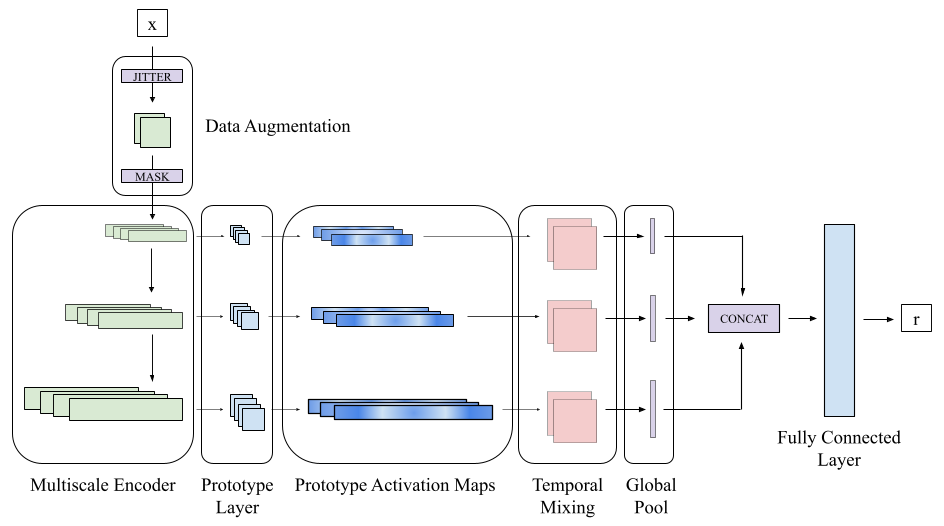
\includegraphics[width = \textwidth]{arch2.png}
    \caption{Generic ProtoTSRL architecture with three segments, though arbitrarily many segments can be linked together in this fashion. Note that the data augmentation block preceding the encoder is only activated during training.}
    \label{fig:arch}
\end{figure}

Figure \ref{fig:arch} summarizes our model architecture. We use a multiscale convolutional encoder $f$ composed of sequential segments $\mathcal S$ where each segment consists of one or more 1D convolutional layers. Early segments use dense or weakly dilated convolutions to capture local morphological details while deeper segments dilate exponentially to expand the receptive field and encode long-range temporal dynamics. Let $f_{\t_i}^{(i)}$ denote the $i^{\text{th}}$ segment of the convolutional encoder parametrized by $\t_i$, and let $f_{\t_{\text{conv}}}$ denote the entire convolutional encoder parametrized by $\t_{\text{conv}}$ with $L$ segments:
\begin{align*}
    f_{\t_{\text{conv}}} = f_{\t_L}^{(L)} \circ \dots \circ f_{\t_2}^{(2)} \circ f_{\t_1}^{(1)}
\end{align*}

Unlike a standard prototype network with a single prototype layer at the end of the encoder, we insert prototype comparisons between encoder segments. Let $x \in \R^{T \times F}$ be a potentially multivariate time series. Denote the latent embedding after segment $\ell \in \mathcal S$ by $z_\ell(x) \in \R^{T_\ell \times F_\ell}$ where 
\begin{align*}
    z_\ell(x) = f_{\t_\ell}^{(\ell)} \circ \dots \circ f_{\t_1}^{(1)}(x)
\end{align*}

We attach a prototype bank $P_\ell = \{ p_1^{(\ell)}, \dots, p_{M_\ell}^{(\ell)} \}$ after the $\ell^{\text{th}}$ segment where each prototype $p_m^{(\ell)} \in \R^{W_\ell \times F_\ell}$ is a learnable patch in the space of $z_\ell$ with $W_\ell \leq T_\ell$. The shallow prototype banks are intended to capture local morphological patterns, while deeper prototype banks capture longer-range temporal motifs in more contextual latent spaces. This yields a sequential prototype model in which different encoder depths correspond to different temporal scales of explanation.

For each prototype $p_m^{(\ell)}$, we compute its inverted cosine similarity to each patch in $z_\ell(x)$, forming an activation map $a_m^{(\ell)}(x) \in \R^{T_\ell}$. In another deviation from a standard prototype network, we do not perform global max pooling over $a_m^{(\ell)}(x)$. Instead, the model preserves the full activation map of every prototype and learns the final representation from the temporal evolution of these prototype responses. This lets the representation retain information not only about whether a pattern occurs, but also about how prototype evidence is organized across time and across scales. Collecting the activation maps of all prototypes at that depth gives the prototype activation tensor:
\begin{align*}
    A^{(\ell)}(x) = 
    \begin{bmatrix}
        a_1^{(\ell)}(x) \\ \vdots \\ a_{M_\ell}^{(\ell)}(x)
    \end{bmatrix}
    \in \R^{M_\ell \times T_\ell}
\end{align*}

We reiterate that because deeper prototype layers operate on features with larger receptive fields, activations in later layers already reflect similarity to longer subseries in the original input. Thus, temporal dynamics are represented jointly by the encoder's multiscale receptive fields and by the time-varying prototype activation maps.

For each prototype layer $\ell$, the prototype activation tensor $A^{(\ell)}(x)$ is treated as a multichannel temporal signal whose channels correspond to learned prototypes. We then apply a temporal convolution module $g^{(\ell)}_{\psi}: \R^{M_\ell \times T_\ell} \to \R^{C_\ell \times T_\ell'}$ to the activation tensor where $C_\ell$ is the number of output channels for that layer and $T_\ell'$ is the resulting length. A separate temporal convolution module is used for each prototype layer to accommodate differences in prototype count, temporal resolution, and receptive-field scale across depths. The purpose of this module is to learn temporal patterns over prototype responses. Since the input channels are prototype activation maps, the temporal convolution mixes across both the channel dimension and the temporal dimension. Therefore, each output channel can capture patterns such as co-activation of multiple prototypes, short-range ordering of prototype responses, repeated prototype activity, or scale-specific temporal motifs expressed in the prototype space. Because the convolution operates on prototype maps rather than on uninterpretable hidden features, the resulting temporal features remain grounded in prototype-based evidence. Lastly, to obtain a single-channel output from layer $\ell$, we apply an adaptive pooling operation over the temporal dimension which we denote as $\text{Pool}_\ell: \R^{C_\ell \times T_\ell'} \to \R^{C_\ell}$, yielding 
\begin{align*}
    b^{(\ell)}(x) = \left(\text{Pool}_\ell \circ g^{(\ell)}_{\psi} \circ A^{(\ell)}\right) (x)
\end{align*}

We concatenate the outputs of all prototype layers: 
\begin{align*}
    u(x) = \left[ b^{(1)}(x); \ldots; b^{(L)}(x) \right]
\end{align*}

A linear projection head maps $u(x)$ to the final representation: 
\begin{align*}
    h(x) = W u(x) + b
\end{align*}

\subsection{Contrastive Learning Framework}
\label{subsec:loss}

\paragraph{Sampling} Let $x^{(i)} \in \R^{T_i \times F}$ denote a potentially multivariate time series and let $x_{\text{anc}}^{(i)}, x_{\text{pos}}^{(i)}, x_{\text{mid}}^{(i)} \subset x^{(i)}$ be temporally contiguous subseries of $x^{(i)}$ where $x_{\text{anc}}^{(i)}$ and $x_{\text{pos}}^{(i)}$ are overlapping and $x_{\text{mid}}^{(i)}$ is distinct from $x_{\text{anc}}^{(i)}$ and $x_{\text{pos}}^{(i)}$. We independently perturb each of these subseries via jittering (prior to encoding) and masking (after the first encoder segment) to produce related contexts $\tilde x_{\text{anc}}^{(i)}, \tilde x_{\text{pos}}^{(i)}, \tilde x_{\text{mid}}^{(i)}$. We consider $\tilde x_{\text{anc}}^{(i)}$ to be the anchor, $\tilde x_{\text{pos}}^{(i)}$ the positive example, and $\tilde x_{\text{mid}}^{(i)}$ the mid-near example (i.e. it is less similar to the anchor than an overlapping view, but it is still more related than a sample drawn from a different series). This intermediate relation is inspired by PaCMAP's distinction between neighbors, mid-near points, and further points, which is used there to balance local and global geometric structure. Here, the same idea is adapted to contrastive learning where intermediate pairs are used to improve the model's learned notion of similarity. Negative examples are sampled from other time series in the minibatch during training and denoted $\tilde x_{\text{neg}}^{(i, j)}$ where $j \neq i$ denotes the series from which it was sampled. Note that while examples do not have to be the same length, care must be taken to ensure that the dimensionality of intermediate embeddings is compatible with prototype layers. In this work, all examples within a batch are the same size for code simplicity, but batches themselves are constructed with samples of different lengths to ensure that the model learns robust representations across different series lengths. 

\paragraph{Prototype Learning} The first role of training is to shape the prototype spaces so that related subseries induce similar prototype responses. Because the model preserves the full activation map of each prototype, prototype similarity is defined at the level of these activation tensors rather than only pooled scalar scores. Let $s(x, y)$ be the cosine similarity between vectors $x$ and $y$: 
\begin{align*}
    s(x, y) = \frac{\langle x, y \rangle}{\| x \|_2 \| y \|_2}
\end{align*}

As before, let $A^{(\ell)}(x)$ be the prototype activation tensor of input
$x$ at layer $\ell$. We define the $\ell$-prototype-space similarity between two series $x$ and $y$ to be the cosine similarity between their flattened prototype activation tensors $\overline A^{(\ell)}(x)$ and $\overline A^{(\ell)}(y)$: 
\begin{align*}
    s_{\text{proto}}^{(\ell)}(x, y) = s\left( \overline A^{(\ell)}(x), \overline A^{(\ell)}(y) \right)
\end{align*}

Two subseries are similar in a prototype space when they induce similar time-varying prototype activation patterns. Using this similarity, we define pair-specific losses for positive, mid-near, and negative relations:
\begin{align*}
    \mathcal L_{\text{pos}}(s) = 1 - s,  \qquad \mathcal L_{\text{mid}}(s) = 0.5(1-s), \qquad \mathcal L_{\text{neg}}(s) = \max(0, s - 0.1)
\end{align*}

Overall, for a training example $x^{(i)}$ from which we sample the anchor $\tilde x_{\text{anc}}^{(i)}$, a positive example $\tilde x_{\text{pos}}^{(i)}$, a mid-near example $\tilde x_{\text{mid}}^{(i)}$, and negative examples $\tilde x_{\text{neg}}^{(i, j)}$ where$j \neq i$ and $N_i$ indexes the minibatch, the loss for layer $\ell$ is
\begin{align*}
    \mathcal L_{\text{proto}}^{(\ell)}(x^{(i)}) = \mathcal L_{\text{pos}} \left(s_{\text{proto}}^{(\ell)} \left(\tilde x_{\text{anc}}^{(i)}, \tilde x_{\text{pos}}^{(i)}\right)\right) + \mathcal L_{\text{mid}}\left(s_{\text{proto}}^{(\ell)}\left(\tilde x_{\text{anc}}^{(i)}, \tilde x_{\text{mid}}^{(i)}\right)\right) + \frac{1}{|N_i|} \sum_{j \in N_i} \mathcal L_{\text{neg}}\left(s_{\text{proto}}^{(\ell)}\left(\tilde x_{\text{anc}}^{(i)}, \tilde x_{\text{neg}}^{(i, j)}\right)\right)
\end{align*}

Because prototypes within the same layer should represent distinct latent components, we additionally include a diversity regularizer that penalizes prototypes that are too similar to one another. This penalty discourages prototype collapse and encourages each prototype bank to span a diverse set of prototypical temporal components. Let $p_a^{(\ell)}$ and $p_b^{(\ell)}$ denote two distinct prototypes in layer $\ell$ (flattened if needed), and define their similarity as the cosine similarity between them:
\begin{align*}
    r_{\text{proto}}^{(\ell)}(a, b) = s\left(p_a^{(\ell)}, p_b^{(\ell)}\right)
\end{align*}

The overall prototype diversity penalty for layer $\ell$ is defined as the average pairwise similarity across all prototypes:
\begin{align*}
    \mathcal R_{\text{div}}^{(\ell)} = \frac{1}{M_\ell (M_\ell - 1)} \sum_{a \neq b} \max \left(0, r_{\text{proto}}^{(\ell)}(a, b) - 0.2\right)
\end{align*}

Over a batch $B$, the objective across all prototype spaces is 
\begin{align}
    \mathcal L_{\text{proto}} = \frac{1}{|B|} \sum_{i \in B} \sum_{\ell \in \mathcal S} \mathcal L_{\text{proto}}^{(\ell)}(x^{(i)}) + \lambda_{\text{proto}} \sum_{\ell \in \mathcal S} \mathcal R_{\text{div}}^{(\ell)}
\end{align}

\paragraph{Representation Learning} After the temporal convolution modules transform the prototype activation maps into fixed-length descriptors, the second role of training is to learn a final representation that preserves the same positive/mid-near/negative ordering. Let $h(x) \in \R^d$ denote the final representation produced by the linear head. We again use cosine similarity: 
\begin{align*}
    s_{\text{repr}}(x, y) = s\left(h(x), h(y)\right)
\end{align*}

In contrast to the prototype-space objective, we use a modified exponential loss to shape the representation space: 
\begin{align*}
    \mathcal L_{\text{repr}}(x^{(i)}) = -\log \left[ \frac{\exp \left( s_{\text{repr}} \left(\tilde x_{\text{anc}}^{(i)}, \tilde x_{\text{pos}}^{(i)}\right) \right)}{\exp \left( s_{\text{repr}} \left(\tilde x_{\text{anc}}^{(i)}, \tilde x_{\text{pos}}^{(i)}\right) \right) + \sum_{j \in N_i} \exp \left( s_{\text{repr}} \left(\tilde x_{\text{anc}}^{(i)}, \tilde x_{\text{neg}}^{(i, j)}\right) \right)} \right] + 0.5\left[1 - s_{\text{repr}} \left(\tilde x_{\text{anc}}^{(i)}, \tilde x_{\text{mid}}^{(i)}\right)\right]
\end{align*}

The exponential loss in the first term is a common choice for contrastive learning (e.g. \cite{eldele21-tstcc,yue21-ts2vec}), and in the vanilla contrastive approach where we only consider positive and negative examples, optimizing this loss maximizes a lower bound on mutual information between paired views \cite{vandenoord19-cpc}. The second term adds a weaker attractive constraint for the mid-near sample rather than treating it as a negative competitor. This modification does not maintain the mutual-information bound for the entire objective, but it preserves the intended geometry of the representation space: positives are pulled together strongly, negatives are contrasted repulsively through the softmax denominator, and mid-near samples are encouraged to remain similar but under a looser constraint.

Since the final representation is generated by a linear layer, we additionally impose $L_1$ regularization on the linear weights to control complexity and discourage over-reliance on a small subset of prototype-derived features. The full representation-space objective over a batch $B$ is therefore 
\begin{align}
    \mathcal L_{\text{repr}} = \frac{1}{|B|} \sum_{i \in B} \mathcal L_{\text{repr}}(x^{(i)}) + \lambda_{\text{repr}} \| W \|_1
\end{align}

We shape the final representation space and the intermediate prototype spaces with different objectives because these stages serve different roles. The intermediate prototype losses are intended to organize the latent spaces around interpretable and diverse prototype activation patterns. This is a more complex structural goal than standard batch discrimination, particularly when a third class of contrasting examples (mid-near samples) are included, and exponential losses are not well-suited for this task due to their emphasis on hard negatives. By contrast, the final representation head is responsible for producing a compact embedding that is globally discriminative within the minibatch. At that stage, an exponential loss is more appropriate.

\subsection{Training}
\label{subsec:training}

We optimize the model in three stages, following the staged training philosophy of ProtoPNet while adapting it to our contrastive framework. ProtoPNet separates learning a meaningful prototype-structured latent space from optimization of the final layer; we adopt the same idea here, but with unsupervised positive, mid-near, and negative relations rather than labeled classes.

\paragraph{Stage 1} In the first stage, we train the encoder and all prototype banks. This can be understood as a pretraining stage guided by the optimization 
\begin{align*}
    \min_{\t_{\text{conv}}, \Phi} \mathcal L_{\text{proto}}
\end{align*}

where $\Phi = \{P_\ell\}_{\ell \in \mathcal S}$ denotes all prototype parameters. This stage shapes the multiscale latent spaces so that related subseries produce similar prototype activation maps at each prototype depth, while the diversity regularizer encourages each prototype bank to learn a non-redundant set of prototypical temporal components.

\paragraph{Stage 2} In the second stage, we freeze the encoder and prototype layers and train the temporal convolution modules together with the final linear head, guided by the optimization 
\begin{align*}
    \min_{\Psi, W} \mathcal L_{\text{repr}}
\end{align*}

where $\Psi = \{\psi^{(\ell)}\}_{\ell \in \mathcal S}$ denotes the parameters of the temporal convolution modules $\{g_{\psi}^{(\ell)}\}_{\ell \in \mathcal S}$. Because prototypes are fixed, this stage learns how to transform and aggregate multiscale prototype activation trajectories into a useful fixed-length representation without altering the prototype structure learned in Stage 1.

\paragraph{Stage 3} In the final stage, we unfreeze the entire network and jointly optimize all parameters:
\begin{align*}
    \min_{\t_{\text{conv}}, \Phi, \Psi, W} \mathcal L_{\text{repr}}
\end{align*}

This final fine-tuning stage allows the encoder, prototypes, temporal readout modules, and linear head to co-adapt while starting from a prototype-structured initialization. Note that the objective for this stage does not contain a prototype regularization term -- if the hyperparameter for number of prototypes was initially misspecified (i.e. a prototype layer can adequately represent the data with fewer prototypes), this stage permits some prototypes to collapse, and these prototypes can be pruned downstream.

% %%%%%%%%% EXPERIMENTS %%%%%%%%%

\section{Experiments}
\label{sec:experiments}

We train ProtoTSRL on several sets of labeled univariate and multivariate time series and evaluate the model's training dynamics, the geometry of the representation space, and the quality of the representations. In particular, we are interested in how each prototype space evolves over the course of training with respect to prototype diversity in that layer. The geometry of the representation space can be visualized with DR (we use PaCMAP), and representation quality is evaluated with classification-based downstream tasks. 

\subsection{Synthetic Time Series}
\label{subsec:synthetic_univariate}

In this section, we create three synthetic datasets -- two univariate and one multivariate -- to test the model's ability to represent and distinguish important characteristics of time series such as periodicity, stationarity, and temporal dependence. Each dataset consists of variable-length time series simulated by one of several user-defined generative processes. To ensure sufficient diversity within the generated data, we add small perturbations to the parameters of each generative process so that each sample is parametrized slightly differently but can still be said to belong to a specific class. For simplicity, these perturbations are applied only to the univariate generative processes. The same model architecture is trained for both univariate datasets: it implements four encoder segments: the first two are dense, so their respective prototype layers learn localized features, while the last two dilate exponentially, so their prototype layers learn longer-term features. A nearly identical architecture is trained for the multivariate dataset, but the prototype layers are larger to improve representation capacity. All representations have 300 features. To evaluate the learned representations, we fit several models of varying complexity -- logistic regression (LR), decision tree (DT), random forest (RF), and multilayer perceptron (MLP) -- to recover the label of the original generative process.

\paragraph{Autoregressive Series} This dataset consists of autoregressive series of order $p$ which we denote as AR($p$): 
\begin{align*}
    x_t = \beta_0 + \sum_{k=1}^p \beta_k x_{t-k} + \epsilon
\end{align*}

where $\epsilon \sim N(0, \sigma^2)$. Each generative process is determined by the parameters $p$ and $\sigma^2$. We enforce all series to be stationary, and we generate three classes with $\sigma^2$ constant: AR(1), AR(5), and AR(10). An example of each class can be found in Figure \ref{fig:autoregressive_data_examples}.

\begin{figure}
    \centering 
    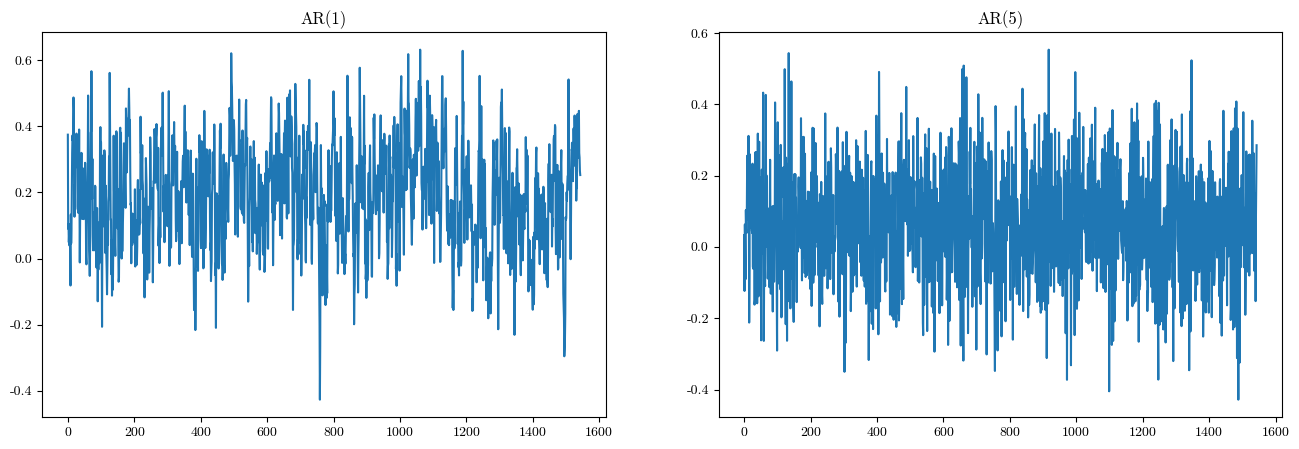
\includegraphics[width = 0.98\textwidth]{autoregressive1.png} \\
    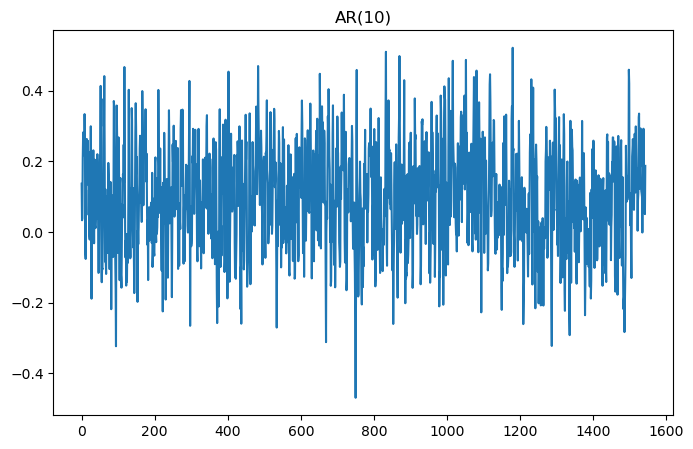
\includegraphics[width = 0.49\textwidth]{autoregressive2.png}
    \caption{Example autoregressive series from each class (AR(1), AR(5), and AR(10)).}
    \label{fig:autoregressive_data_examples}
\end{figure}

We first analyze the evolution of the learned prototype spaces throughout training via the average pairwise similarity between prototypes in each layer. Lower average similarity implies the prototypes are more diverse and further apart within their respective latent space, thereby learning to capture a broader range of morphological structures. We expect prototype similarity to decrease in Stage 1 training due to the prototype regularization component and to remain constant in Stage 2 as prototype layers are frozen. However, in Stage 3, the objective does not regularize prototypes at all, so the behavior of prototype similarity is unknown. These similarities are plotted by training epoch in Figure \ref{fig:autoregressive_univariate_dynamics}. Perhaps predictably, these trajectories indicate that the model quickly prefers to diversify later prototype spaces that represent long-term morphologies. Indeed, even with brief inspection, we notice that these autoregressive series are difficult to distinguish and highly volatile. As such, local morphologies are unlikely to hold much useful information about the temporal dependence structure of the series. However, global training significantly disrupts learned prototypes in all but the last layer, and these disruptions are non-monotone and, in the case of layer 3, volatile. It is likely that this disruption is also due to the uninformative nature of early prototypes -- during global training, they move erratically in the absence of the diversity incentive because there are no informative local morphologies to be found.

\begin{figure}
    \centering
    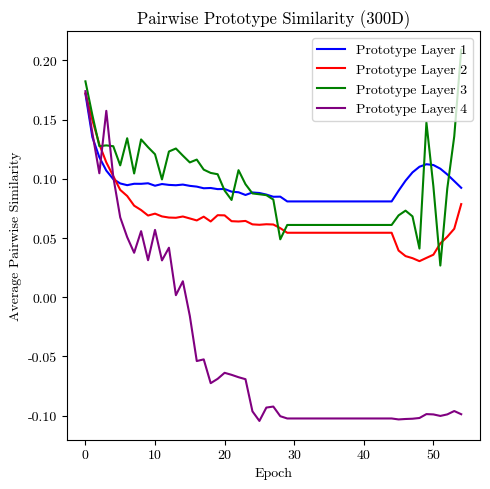
\includegraphics[width = 0.7\textwidth]{autoregressive_univariate_dynamics.png}
    \caption{Average pairwise prototype similarity by layer for autoregressive series representation. These trajectories are flat during Stage 2 training (epochs 31 to 45), and early layer volatility is evident during Stage 3 training (epochs 46-55).}
    \label{fig:autoregressive_univariate_dynamics}
\end{figure}

Because ProtoTSRL learns fixed-length representations, we are additionally able to visualize the representation space directly via DR and evaluate representation quality through the geometry of the learned space. PaCMAP embeddings of autoregressive series representations in two and three dimensions are shown in Figure \ref{fig:autoregression_pacmap}. We include both two and three dimensional embeddings because the geometry of the embedding is not always obvious in two dimensions. From this result, it seems ProtoTSRL is exceptionally good at learning to recognize temporal dependence structure as the representation space achieves perfect separation. The high quality of these representations is reflected in downstream tasks as well: all classifiers learned to predict the original data generating process (i.e. the order $p$ of the autoregression) with perfect accuracy.

\begin{figure}
    \centering 
    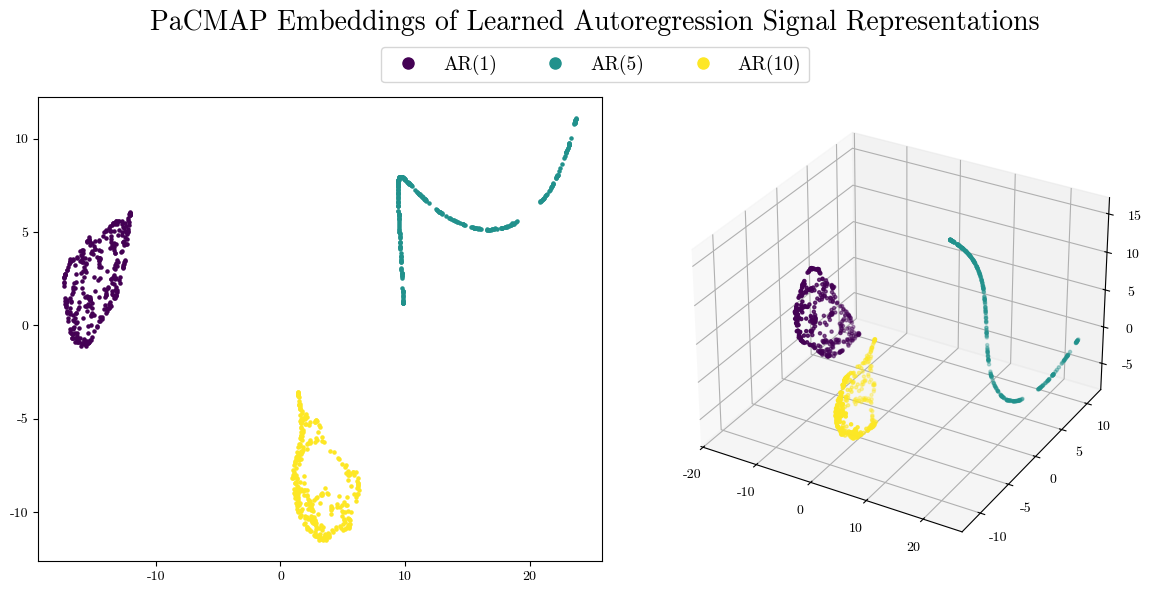
\includegraphics[width = 0.95\textwidth]{autoregressive_univariate_pacmap.png}
    \caption{PaCMAP embeddings of autoregressive series representations in two and three dimensions. These embeddings reflect perfect separation in the representation space.}
    \label{fig:autoregression_pacmap}
\end{figure}

\paragraph{Periodic Series} This dataset consists of periodic (sinusoidal) series. The data generative process is determined by two components: wave parameters (frequency, amplitude, vertical shifts, phase shifts, drift) and noise parameters (amplitude jittering, frequency jittering, additive Gaussian noise, baseline wander). We generate five classes: (1) base sine wave, (2) base sine wave with different frequency and amplitude, (3) sine wave with positive linear drift, (4) sine wave with negative linear drift, (5) sine wave with positive vertical shift. The same noise parameters are applied to all 5 classes. An example of each class can be found in Figure \ref{fig:periodic_data_examples}.

\begin{figure}
    \centering 
    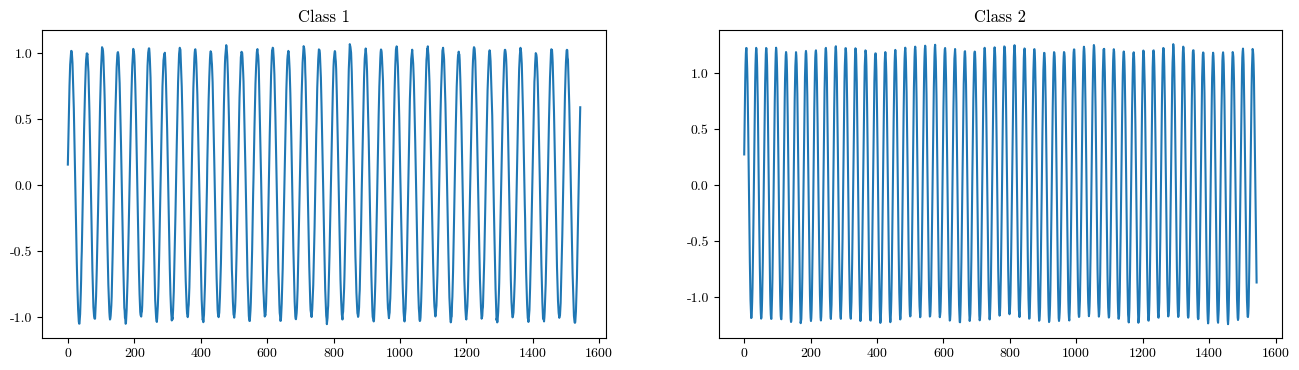
\includegraphics[width = 0.98\textwidth]{periodic1.png} \\
    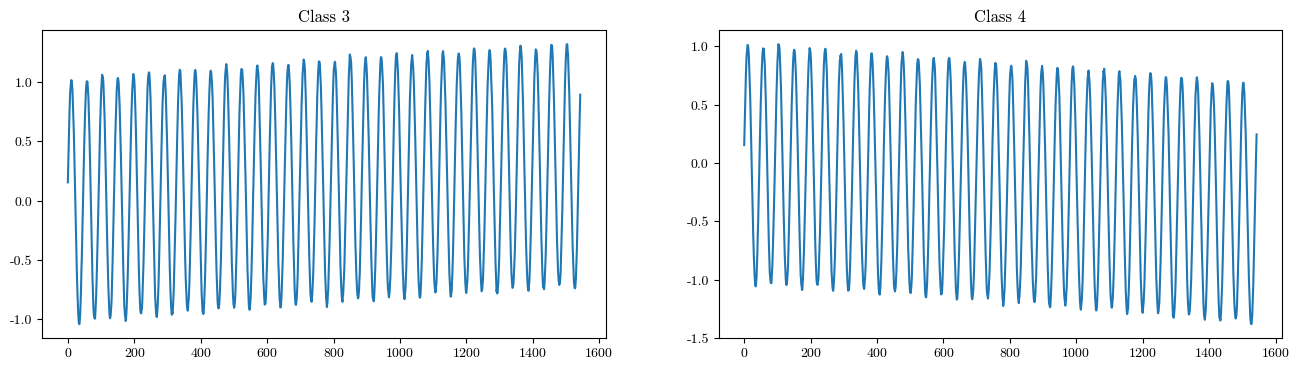
\includegraphics[width = 0.98\textwidth]{periodic2.png} \\
    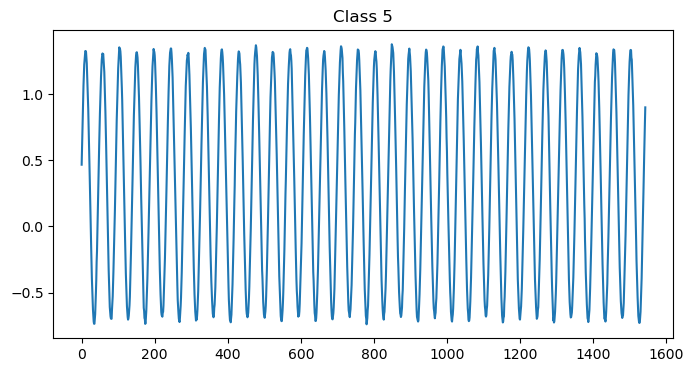
\includegraphics[width = 0.49\textwidth]{periodic3.png}
    \caption{Example periodic series from each class.}
    \label{fig:periodic_data_examples}
\end{figure}

Prototype similarities at each layer are shown in Figure \ref{fig:periodic_univariate_dynamics}. These trajectories also indicate that the model quickly prefers to diversify later prototype spaces that represent long-term morphologies. For highly periodic series, we again hypothesize that local morphologies are unlikely to hold much unique information as they are more prone to corruption due to added noise. However, it appears that global training challenges this hypothesis: in final epochs, the earliest prototype layer becomes significantly more diverse while later ones are approximately fixed. It is unclear why this is the case -- some wave parameters (i.e. frequency and amplitude) may be detectable locally, but this should affect the prototype space in Stage 1 as well as Stage 3. 

\begin{figure}
    \centering 
    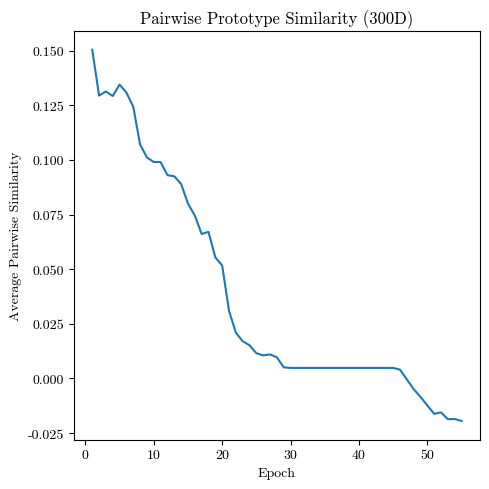
\includegraphics[width = 0.7\textwidth]{periodic_univariate_dynamics.png}
    \caption{Average pairwise prototype similarity by layer for periodic series representation. Early layer diversification is evident during Stage 3 training (epochs 46-55).}
    \label{fig:periodic_univariate_dynamics}
\end{figure}

PaCMAP embeddings of periodic series representations in two and three dimensions are shown in Figure \ref{fig:periodic_pacmap}. The three dimensional visualization is of particular importance. ProtoTSRL clearly distinguishes series by frequency and amplitude (class 2). On the other hand, positive linear drift is only partly distinguished, and it overlaps significantly with positive vertical shift (class 5). There is also separation between the base series and negative linear drift (classes 1 and 4). The two are separable, but their embeddings are intertwined. Many of these nuances are only evident in three dimensions: the two dimensional embedding mixes classes together, but this is not reflective of manifold geometry. 

\begin{figure}
    \centering 
    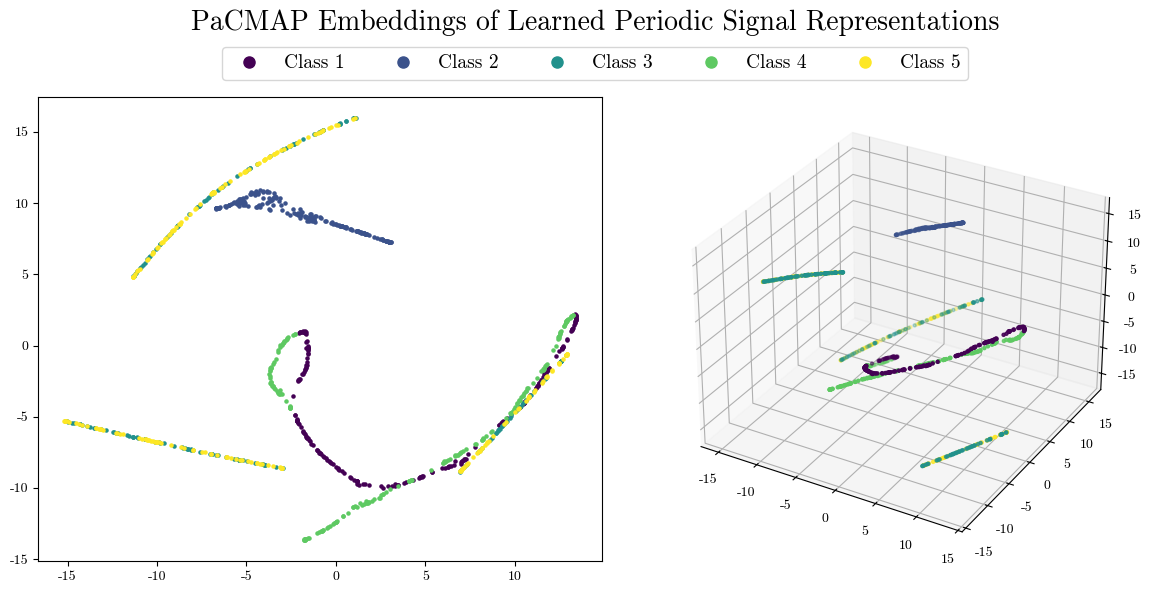
\includegraphics[width = 0.95\textwidth]{periodic_univariate_pacmap.png}
    \caption{PaCMAP embeddings of periodic series representations in two and three dimensions.}
    \label{fig:periodic_pacmap}
\end{figure}

Lastly, we evaluate representation quality. Model accuracies are listed in Table \ref{tab:periodic_model_accuracies}. The strong performance of these models indicate that the learned representations indeed captured important semantic information about the underlying series. Moreover, in conjunction with the representation space visualizations provided by PaCMAP, these results suggest that perfect class separation in the representation space is not a precondition for effective information preservation. Despite the mixing of various classes present in the DR embeddings, even simple models were able to learn a highly accurate decision boundary that distinguishes between different latent generative processes. 

\begin{table}[ht]
\centering
\renewcommand{\arraystretch}{1.6}
\setlength{\tabcolsep}{5pt}
\begin{tabular}
    {p{0.1\textwidth} p{0.20\textwidth} p{0.20\textwidth} p{0.20\textwidth} p{0.20\textwidth}}
    & \centering\textbf{Logistic Regression} & \centering\textbf{Decision Tree} & \centering\textbf{Random Forest} & \centering\arraybackslash\textbf{Multilayer Perceptron} \\[0.8em]
    \hline
    \textbf{Accuracy}
    & \centering 0.952 & \centering 0.964 & \centering 0.982 & \centering\arraybackslash 0.964 \\
    [0.6em]
\end{tabular}
\vspace{0.8em}
\caption{Model accuracies in classification of periodic series representations.}
\label{tab:periodic_model_accuracies}
\end{table}

To understand model performance and representation quality in greater detail, we also include the confusion matrix of the MLP in Table \ref{tab:periodic_nlp_confusion_matrix}. As we saw before, classes 3 and 5 are difficult to distinguish and yield incorrect classifications. However, other classes which appeared to be difficult to separate in the representation space are well-classified here. 

\begin{table}[ht]
    \centering
    \renewcommand{\arraystretch}{1.6}
    \setlength{\tabcolsep}{12pt}
    \begin{tabular}
        {p{0.16\textwidth} | p{0.12\textwidth} p{0.12\textwidth} p{0.12\textwidth} p{0.12\textwidth} p{0.12\textwidth}}
        & \centering\textbf{Predicted Class 1} 
        & \centering\textbf{Predicted Class 2} 
        & \centering\textbf{Predicted Class 3} 
        & \centering\textbf{Predicted Class 4} 
        & \centering\arraybackslash\textbf{Predicted Class 5} \\[0.8em]
        \hline
        \textbf{Actual Class 1} & \centering 210 & \centering 0 & \centering 0 & \centering 0 & \centering\arraybackslash 0 \\[0.6em]
        \textbf{Actual Class 2} & \centering 0 & \centering 185 & \centering 0 & \centering 0 & \centering\arraybackslash 0 \\[0.6em]
        \textbf{Actual Class 3} & \centering 0 & \centering 0 & \centering 170 & \centering 0 & \centering\arraybackslash \textcolor{red}{26} \\[0.6em]
        \textbf{Actual Class 4} & \centering 0 & \centering 0 & \centering 0 & \centering 200 & \centering\arraybackslash 0 \\[0.6em]
        \textbf{Actual Class 5} & \centering 0 & \centering 0 & \centering \textcolor{red}{9} & \centering 0 & \centering\arraybackslash 200 \\[0.6em]
    \end{tabular}
    \vspace{0.8em}
    \caption{Confusion matrix for classification of periodic series representations with MLP. Incorrect predictions are highlighted in red.}
    \label{tab:periodic_nlp_confusion_matrix}
\end{table}








%%%%%%%%%%%%%%%

\paragraph{Vector Autoregression Series} autoregressive series of order $p$ which we denote as VAR($d, p$) where $d$ is the feature dimensionality of the series and $p$ is the order of the temporal dependence as before:
\begin{align*}
    \mathbf{x_t} = A_0 + \sum_{k=1}^p A_k \mathbf{x_{t-k}} + \mathbf \epsilon
\end{align*}

where $A_0 \in \mathbb R^d$, $A_k \in \mathbb R^{d \times d}$ for all $1 \leq k \leq p$, and $\epsilon \sim MVN(\mathbf \mu, \Sigma^2)$. We choose $d = 4$ and omit it in future notation. This dataset consists of three generating processes: VAR(1), VAR(5), and VAR(10). We again enforce stationarity, but the parameters of each process are all distinct. An example of VAR(10) plotted channel-wise can be found in Figure \ref{fig:var_data_examples}.

\begin{figure}
    \centering 
    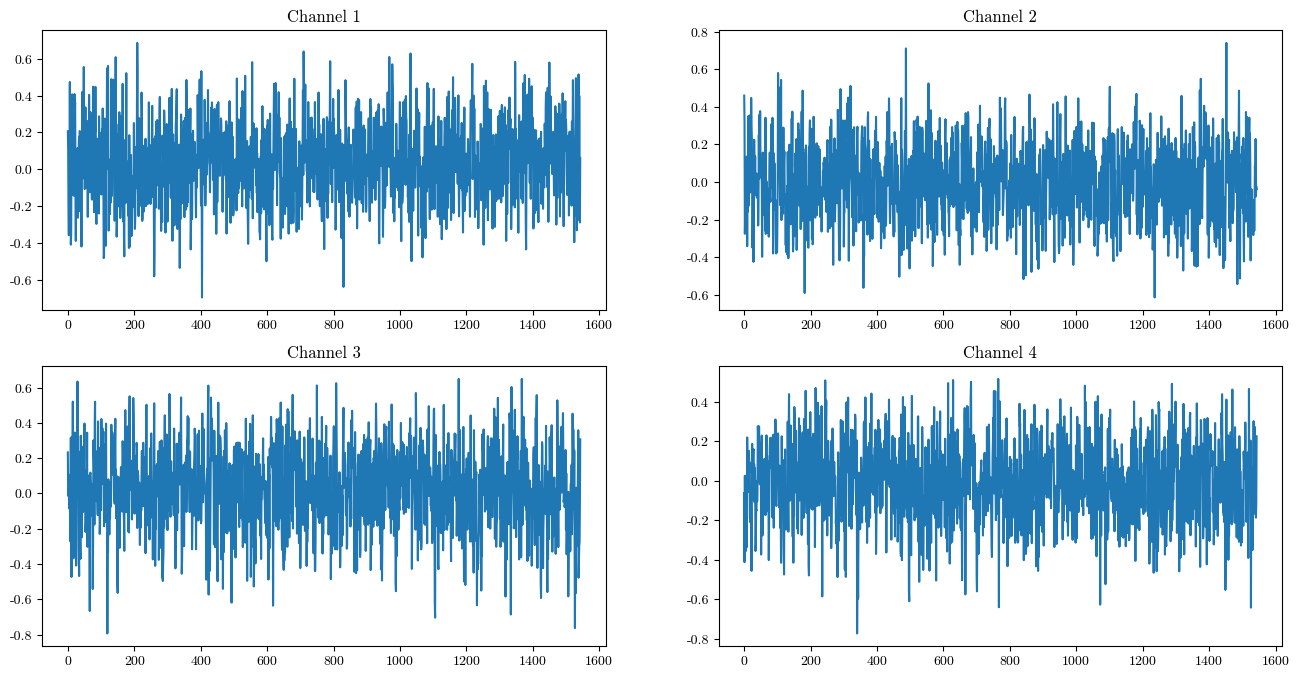
\includegraphics[width = \textwidth]{var.png}
    \caption{VAR(10) sample series plotted by channel.}
    \label{fig:var_data_examples}
\end{figure}

[BOOKMARK] Prototype similarities at each layer are shown in Figure \ref{fig:periodic_univariate_dynamics}. These trajectories also indicate that the model quickly prefers to diversify later prototype spaces that represent long-term morphologies. For highly periodic series, we again hypothesize that local morphologies are unlikely to hold much unique information as they are more prone to corruption due to added noise. However, it appears that global training challenges this hypothesis: in final epochs, the earliest prototype layer becomes significantly more diverse while later ones are approximately fixed. It is unclear why this is the case -- some wave parameters (i.e. frequency and amplitude) may be detectable locally, but this should affect the prototype space in Stage 1 as well as Stage 3. 

\begin{figure}
    \centering 
    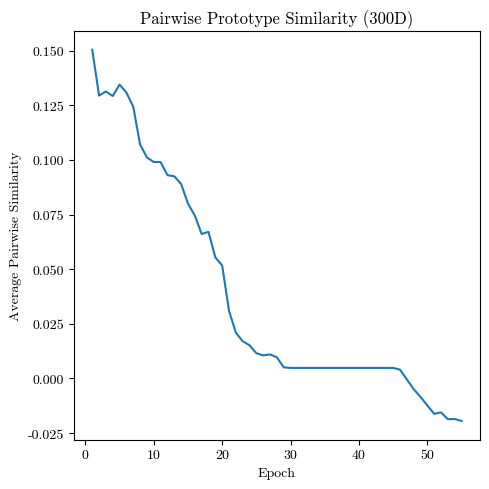
\includegraphics[width = 0.7\textwidth]{periodic_univariate_dynamics.png}
    \caption{Average pairwise prototype similarity by layer for periodic series representation. Early layer diversification is evident during Stage 3 training (epochs 46-55).}
    \label{fig:periodic_univariate_dynamics}
\end{figure}

PaCMAP embeddings of periodic series representations in two and three dimensions are shown in Figure \ref{fig:periodic_pacmap}. The three dimensional visualization is of particular importance. ProtoTSRL clearly distinguishes series by frequency and amplitude (class 2). On the other hand, positive linear drift is only partly distinguished, and it overlaps significantly with positive vertical shift (class 5). There is also separation between the base series and negative linear drift (classes 1 and 4). The two are separable, but their embeddings are intertwined. Many of these nuances are only evident in three dimensions: the two dimensional embedding mixes classes together, but this is not reflective of manifold geometry. 

\begin{figure}
    \centering 
    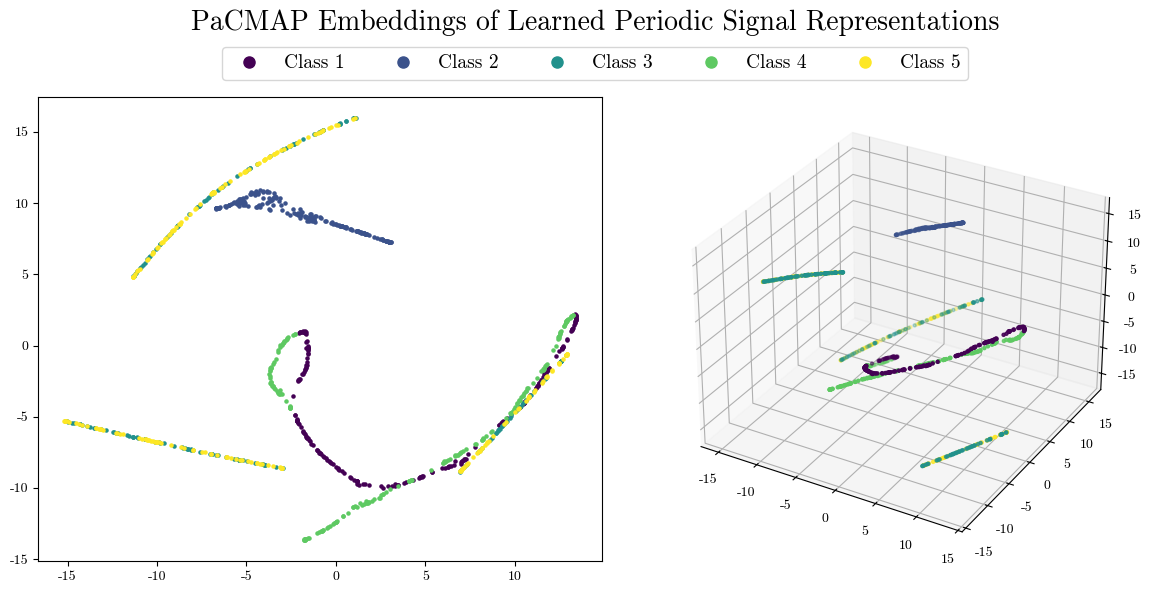
\includegraphics[width = 0.95\textwidth]{periodic_univariate_pacmap.png}
    \caption{PaCMAP embeddings of periodic series representations in two and three dimensions.}
    \label{fig:periodic_pacmap}
\end{figure}

Lastly, we evaluate representation quality. Model accuracies are listed in Table \ref{tab:periodic_model_accuracies}. The strong performance of these models indicate that the learned representations indeed captured important semantic information about the underlying series. Moreover, in conjunction with the representation space visualizations provided by PaCMAP, these results suggest that perfect class separation in the representation space is not a precondition for effective information preservation. Despite the mixing of various classes present in the DR embeddings, even simple models were able to learn a highly accurate decision boundary that distinguishes between different latent generative processes. 

\begin{table}[ht]
\centering
\renewcommand{\arraystretch}{1.6}
\setlength{\tabcolsep}{5pt}
\begin{tabular}
    {p{0.1\textwidth} p{0.20\textwidth} p{0.20\textwidth} p{0.20\textwidth} p{0.20\textwidth}}
    & \centering\textbf{Logistic Regression} & \centering\textbf{Decision Tree} & \centering\textbf{Random Forest} & \centering\arraybackslash\textbf{Multilayer Perceptron} \\[0.8em]
    \hline
    \textbf{Accuracy}
    & \centering 0.952 & \centering 0.964 & \centering 0.982 & \centering\arraybackslash 0.964 \\
    [0.6em]
\end{tabular}
\vspace{0.8em}
\caption{Model accuracies in classification of periodic series representations.}
\label{tab:periodic_model_accuracies}
\end{table}

To understand model performance and representation quality in greater detail, we also include the confusion matrix of the MLP in Table \ref{tab:periodic_nlp_confusion_matrix}. As we saw before, classes 3 and 5 are difficult to distinguish and yield incorrect classifications. However, other classes which appeared to be difficult to separate in the representation space are well-classified here. 

\begin{table}[ht]
    \centering
    \renewcommand{\arraystretch}{1.6}
    \setlength{\tabcolsep}{12pt}
    \begin{tabular}
        {p{0.16\textwidth} | p{0.12\textwidth} p{0.12\textwidth} p{0.12\textwidth} p{0.12\textwidth} p{0.12\textwidth}}
        & \centering\textbf{Predicted Class 1} 
        & \centering\textbf{Predicted Class 2} 
        & \centering\textbf{Predicted Class 3} 
        & \centering\textbf{Predicted Class 4} 
        & \centering\arraybackslash\textbf{Predicted Class 5} \\[0.8em]
        \hline
        \textbf{Actual Class 1} & \centering 210 & \centering 0 & \centering 0 & \centering 0 & \centering\arraybackslash 0 \\[0.6em]
        \textbf{Actual Class 2} & \centering 0 & \centering 185 & \centering 0 & \centering 0 & \centering\arraybackslash 0 \\[0.6em]
        \textbf{Actual Class 3} & \centering 0 & \centering 0 & \centering 170 & \centering 0 & \centering\arraybackslash \textcolor{red}{26} \\[0.6em]
        \textbf{Actual Class 4} & \centering 0 & \centering 0 & \centering 0 & \centering 200 & \centering\arraybackslash 0 \\[0.6em]
        \textbf{Actual Class 5} & \centering 0 & \centering 0 & \centering \textcolor{red}{9} & \centering 0 & \centering\arraybackslash 200 \\[0.6em]
    \end{tabular}
    \vspace{0.8em}
    \caption{Confusion matrix for classification of periodic series representations with MLP. Incorrect predictions are highlighted in red.}
    \label{tab:periodic_nlp_confusion_matrix}
\end{table}

%%%%%%%%%%%%%%%%%%%%







\subsection{PPG Signals} We use artificial PPG data generated to train DeepBeat \cite{soto20-deepbeat}. The dataset contains constant-length PPG signal data with varying amounts of noise. Each series is labeled with a binary indicator of whether atrial fibrillation (AFib) occurs at some point within the series. Examples of AFib and normal sinus rhythm (NSR) can be found in Figure \ref{fig:ppg_data_examples}.

\begin{figure}[ht]
    \centering 
    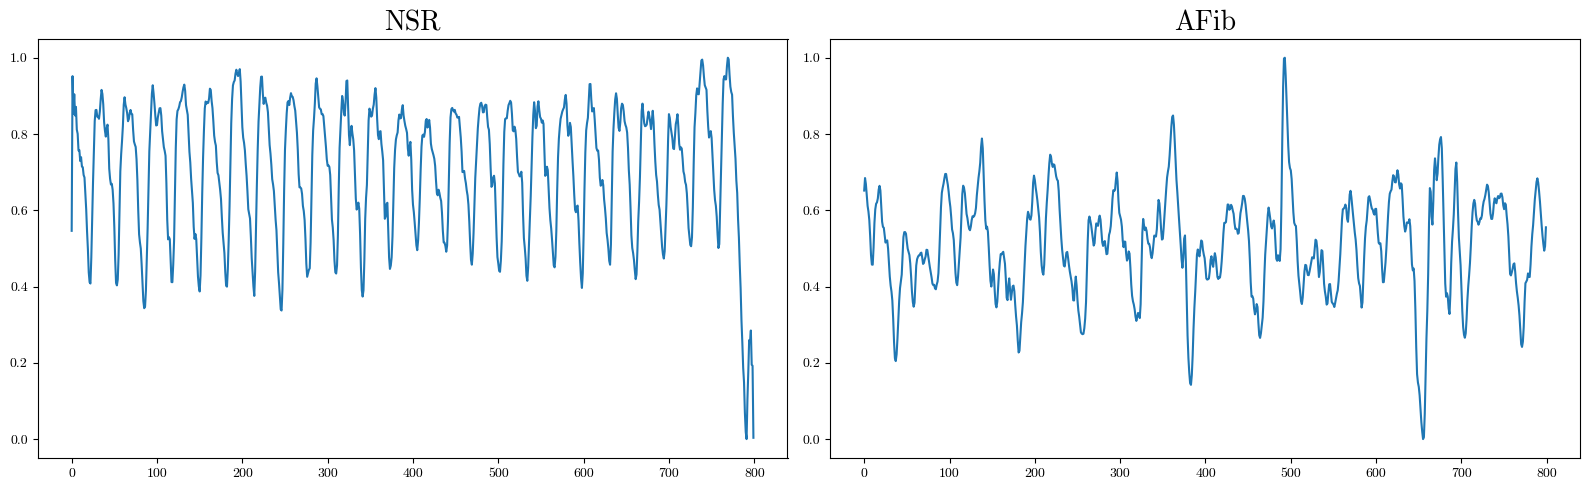
\includegraphics[width = \textwidth]{ppg.png}
    \caption{Example PPG data. Note that both examples are noisy and contain artifacts such as anomalous spikes.}
    \label{fig:ppg_data_examples}
\end{figure}

PaCMAP embeddings of PPG series representations in two and three dimensions are shown in Figure \ref{fig:ppg_deep_pacmap}. Separation in the representation space is not as clean as it was for previous datasets. This could be due in part to the fact that most signals, even if they contain AFib periods, also contain long periods of NSR. As a result, without parameter adjustment or finetuning, the model does not learn to strongly distinguish small anomalies. However, there is still an obvious clustering structure within these embeddings: AFib signals occupy a thin strip along the manifold in the middle of the more expansive NSR signals. 

\begin{figure}
    \centering 
    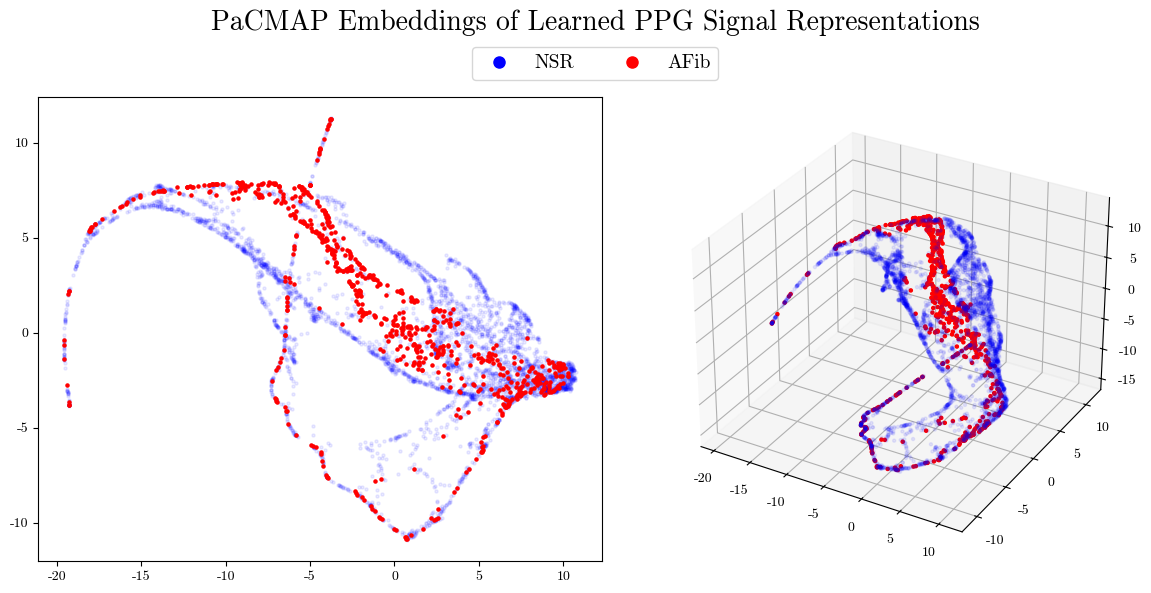
\includegraphics[width = \textwidth]{ppg_deep_pacmap.png}
    \caption{PaCMAP embeddings of PPG series representations in two and three dimensions.}
    \label{fig:ppg_deep_pacmap}
\end{figure}

Given the poor separation in the representation space, it is somewhat expected that downstream models do not perform particularly well in classifying representations of AFib and normal PPG signals (Table \ref{tab:ppg_model_accuracies}). However, the confusion matrix for a multilayer perceptron trained on this classification task (Table \ref{tab:ppg_confusion_matrix}) reveals an interesting characteristic in the model's decisions. Much of the model's error originates from false positives, indicating that the model is highly sensitive to anomalies which may include noise artifacts in the data. In comparison, it makes very few false negative mistakes. 

\begin{table}[ht!]
\centering
\renewcommand{\arraystretch}{1.6}
\setlength{\tabcolsep}{5pt}
\begin{tabular}
    {p{0.1\textwidth} p{0.20\textwidth} p{0.20\textwidth} p{0.20\textwidth} p{0.20\textwidth}}
    & \centering\textbf{Logistic Regression} & \centering\textbf{Decision Tree} & \centering\textbf{Random Forest} & \centering\arraybackslash\textbf{Multilayer Perceptron} \\[0.8em]
    \hline
    \textbf{Accuracy}
    & \centering 0.679 & \centering 0.702 & \centering 0.767 & \centering\arraybackslash 0.626 \\
    [0.6em]
\end{tabular}
\vspace{0.8em}
\caption{Model accuracies in classification of PPG data.}
\label{tab:ppg_model_accuracies}
\end{table}
\vspace{1em}

\begin{table}[ht!]
    \centering
    \renewcommand{\arraystretch}{1.6}
    \setlength{\tabcolsep}{12pt}
    \begin{tabular}
        {p{0.18\textwidth} | p{0.18\textwidth} p{0.18\textwidth}}
        & \centering\textbf{Predicted NSR} & \centering\arraybackslash\textbf{Predicted AFib} \\[0.8em]
        \hline
        \textbf{Actual NSR} & \centering 2918 & \centering\arraybackslash 1613 \\[0.6em]
        \textbf{Actual AFib} & \centering 81 & \centering\arraybackslash 666 \\[0.6em]
    \end{tabular}
    \vspace{0.8em}
    \caption{Confusion matrix for NSR and AFib classification with MLP.}
    \label{tab:ppg_confusion_matrix}
\end{table}

\paragraph{Supervised Finetuning} Time series data is a particularly powerful application for supervised finetuning (SFT) methods given label sparsity. We attempt SFT for the PPG model by appending a single fully connected layer to the end of a stagewise-pretrained network which takes in a learned representation and outputs a logit of the probability that the representation is one of AFib. The goal of SFT in this context is to teach the model to distinguish between relevant and irrelevant artifacts -- the former characterizes AFib while the latter is a remnant of observation methods (e.g. movement while wearing a PPG sensor). We train this entire modified network with cross entropy loss on a small (10\%), labeled subset of the training set. The same jittering and masking augmentations are applied as before, though we do not include the contrastive sampling step for obvious reasons. However, we note that if we had subsequence annotations (i.e. we know exactly where in each series AFib occurs), we could have performed SFT with a supervised contrastive objective. 

The training dynamics of this model from the start of pretraining to the end of SFT is shown in Figure \ref{fig:ppg_deep_dynamics}. In pretraining, this model differs from the models described above by emphasizing diversity in earlier prototype layers. Indeed, AFib signals are often characterized by short-term morphological features such as inconsistent pulse shapes. In contrast, however, normal sinus rhythm (NSR) is a long-term feature characterized by consistent pulses over time. The combination of these two morphologies may explain why layers 2 and 3 are both highly diverse. The effect of global pretraining is not as erratic as in previous examples, though it does reduce the diversity of earlier layers. This trend has been generally true across all datasets -- global training tends to disrupt earlier prototype layers more than later ones. Far more significant prototype disruption occurs during SFT (after epoch 55). The earliest prototype layer immediately begins collapsing, and later layers also lose a degree of diversity. Early layer collapse may be a positive as AFib signals should be morphologically similar across all series. Certain periodicity characteristics may differ due to factors such as the patient's resting heart rate, but AFib itself is defined by rapid, irregular pulse rhythms which should result in similar PPG signals. As such, early layer collapse could mean that the model is learning which local morphologies are characteristic of AFib and discarding those which merely reflect external noise. 

\begin{figure}
    \centering 
    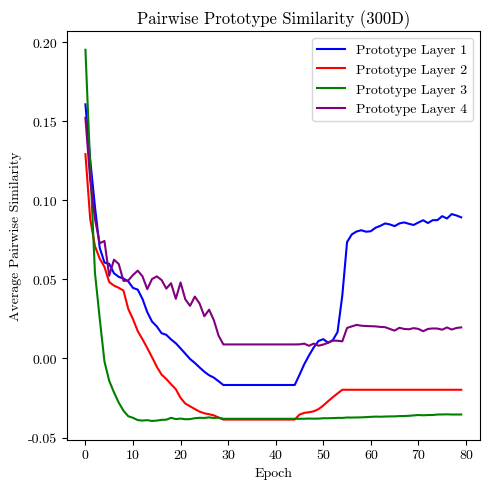
\includegraphics[width = 0.7\textwidth]{ppg_deep_dynamics.png}
    \caption{Average pairwise prototype similarity by layer.}
    \label{fig:ppg_deep_dynamics}
\end{figure}

PaCMAP embeddings of PPG series representations following SFT are shown in Figure \ref{fig:ppg_deep_sft_pacmap}. Evaluated qualitatively, the geometry of the representation space does not change significantly before and after SFT, and class separation does not appear to be improved in any meaningful way. 

\begin{figure}
    \centering 
    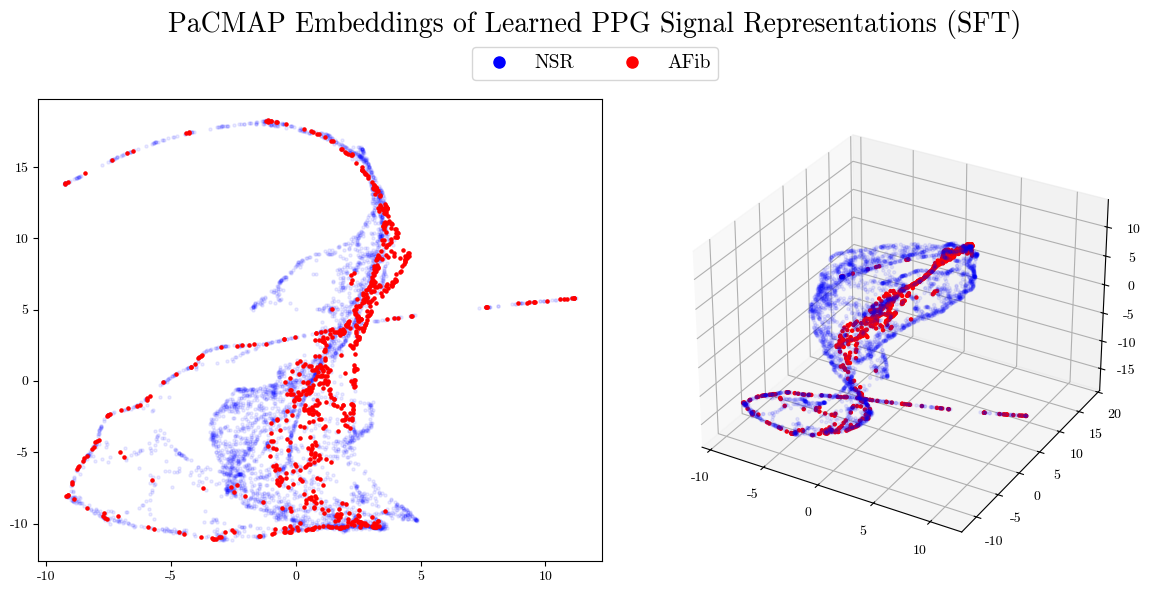
\includegraphics[width = \textwidth]{ppg_deep_sft_pacmap.png}
    \caption{PaCMAP embeddings of PPG series representations after SFT in two and three dimensions. PaCMAP embeddings are rotation invariant, so we compare these embeddings with those of representations generated without SFT by the shape of the embeddings, not the direction from which it is viewed.}
    \label{fig:ppg_deep_sft_pacmap}
\end{figure}

The effect of SFT is more significantly reflected in downstream classification performance (Tables \ref{tab:ppg_sft_model_accuracies} and \ref{tab:ppg_sft_confusion_matrix}). There is a marked reduction in both false positives and false negatives, though the latter was low to begin with. In particular, the reduction in false positives indicates that SFT taught the model to distinguish between true AFib signals and irrelevant noise. We note that our approach to SFT was somewhat naive -- we randomly sampled training examples and passed them to the model without further modification. Even absent subsequence annotations, further augmenting SFT training data via the addition of noise or by rebalancing the dataset in favor of AFib examples may improve subsequent performance. Domain-specific approaches to SFT are a potential direction for future work. 

\begin{table}[ht!]
\centering
\renewcommand{\arraystretch}{1.6}
\setlength{\tabcolsep}{5pt}
\begin{tabular}
    {p{0.1\textwidth} p{0.20\textwidth} p{0.20\textwidth} p{0.20\textwidth} p{0.20\textwidth}}
    & \centering\textbf{Logistic Regression} & \centering\textbf{Decision Tree} & \centering\textbf{Random Forest} & \centering\arraybackslash\textbf{Multilayer Perceptron} \\[0.8em]
    \hline
    \textbf{Accuracy}
    & \centering 0.868 & \centering 0.847 & \centering 0.860 & \centering\arraybackslash 0.856 \\
    [0.6em]
\end{tabular}
\vspace{0.8em}
\caption{Model accuracies in classification of PPG data.}
\label{tab:ppg_sft_model_accuracies}
\end{table}
\vspace{1em}

\begin{table}[ht!]
    \centering
    \renewcommand{\arraystretch}{1.6}
    \setlength{\tabcolsep}{12pt}
    \begin{tabular}
        {p{0.18\textwidth} | p{0.18\textwidth} p{0.18\textwidth}}
        & \centering\textbf{Predicted NSR} & \centering\arraybackslash\textbf{Predicted AFib} \\[0.8em]
        \hline
        \textbf{Actual NSR} & \centering 3778 & \centering\arraybackslash 753 \\[0.6em]
        \textbf{Actual AFib} & \centering 7 & \centering\arraybackslash 740 \\[0.6em]
    \end{tabular}
    \vspace{0.8em}
    \caption{Confusion matrix for NSR and AFib classification with MLP following SFT.}
    \label{tab:ppg_sft_confusion_matrix}
\end{table}

A natural question to ask when employing prototype-based methods is what features are actually being learned. In some architectures (e.g. ProtoPNet), prototypes are explicitly ``pushed'' to their nearest match in the training set. In this way, a prototype learns to represent a literal example in the training set. Rather than pushing prototypes onto training examples, we visualize regions of high activation along the original series. This gives us a sense of what morphologies are represented by each prototype while allowing prototypes to exist potentially as amalgamations of important common structures that are similar but not the same (i.e. a prototype is somewhat close to multiple slightly different training examples rather than representative of one specific motif in a single example). Figure \ref{fig:ppg_proto_act} visualizes activation maps for four different prototypes at different layers in the network. Two prototypes activate strongly on NSR signals while the other two activate on AFib signals. Note that prototypes in later layers activate more smoothly over larger periods, presumably because they capture long-term patterns that manifest over wide ranges of the signal. 

Activation maps like these can often provide valuable domain-specific insights. For example, if we knew nothing about PPG data morphology, we may notice that in the NSR case, early prototypes activate highly on individual peaks while later prototypes activate highly across a long time range. This may suggest that NSR is characterized not only by a specific peak morphology, but by the repetition of this morphology over time. 

\begin{figure}
    \centering
    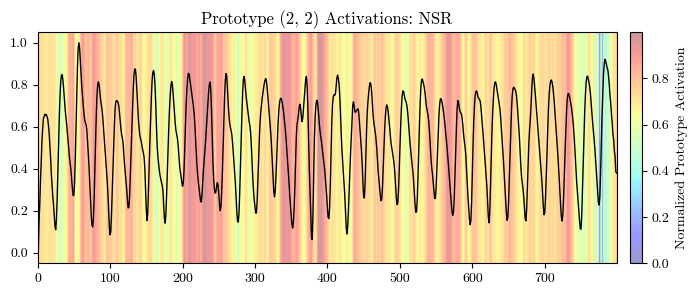
\includegraphics[width = 0.48\textwidth]{nsr_proto22_deep.png}
    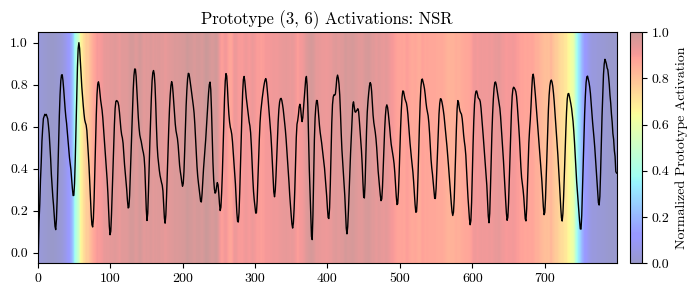
\includegraphics[width = 0.48\textwidth]{nsr_proto36_deep.png} \\
    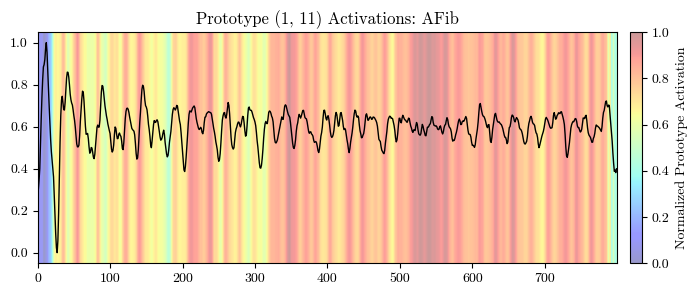
\includegraphics[width = 0.48\textwidth]{afib_proto111_deep.png}
    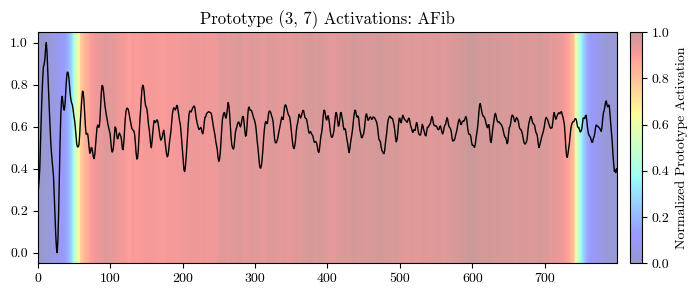
\includegraphics[width = 0.48\textwidth]{afib_proto37_deep.png} 
    \caption{Highly activated prototypes for NSR (top) and AFib (bottom). Each prototype is identified by (layer, index).}
    \label{fig:ppg_proto_act}
\end{figure}

\section{Discussion}
\label{sec:discussion}

Compared with prior self-supervised methods, the reasoning process of ProtoTSRL is substantially more transparent. Intermediate latent spaces are shaped directly by learned prototypes rather than by abstract contrastive objectives, and the model explicitly learns to recognize morphological structure through prototypes which is reminiscent of human reasoning. This provides a more interpretable account of how the model organizes similarity: rather than mapping an input directly into a black-box embedding space, the model first compares it to learned prototypical patterns and then learns temporal relationships among those prototype responses.

This structure also makes it possible to study how the model allocates representational capacity across scales. In our experiments, prototype diversity trajectories suggest a tradeoff between learning diverse local morphologies and diverse long-range temporal structures. For some datasets, the model appears to prioritize later prototype layers, indicating that global temporal behavior is more informative than local shape. In other settings, especially those involving short-term irregularities, earlier prototype layers also remain highly diverse. This behavior is itself informative: it suggests that the model is adapting its prototype spaces to the temporal scale at which distinguishing structure occurs. 

Prototype activation visualizations provide an additional source of insight that is valuable apart from downstream prediction. By identifying regions of high activation along the original series, these visualizations suggest which local motifs or longer-term temporal patterns are most salient to the model. In this sense, the learned prototypes may serve as a tool for exploratory analysis and domain discovery. This is especially useful in domains where meaningful patterns are difficult to describe \textit{a priori} but can be recognized once highlighted in context.

\paragraph{Limitations} Despite these advantages, the present study has several limitations. First, the experiments are not yet sufficiently diverse to fully characterize the strengths and weaknesses of the proposed approach. Although the synthetic datasets are useful for isolating specific properties such as periodicity and temporal dependence, they do not capture the full range of challenges encountered in real-world time series. In particular, we did not construct multivariate toy datasets, which limits our ability to study whether the learned prototypes remain interpretable when meaningful structure depends on interactions across features rather than along a single channel. Since multivariate structure is one of the main motivations for richer representation learning, this remains an important gap.

A further practical limitation is the cost of experimentation. Many standard practices in model development, such as broad hyperparameter tuning, repeated retraining, or large-scale architecture search, are difficult in this setting because both training and inference can be expensive. As a result, some potentially important design questions, such as the optimal number of prototypes per layer, the best receptive-field schedule, or the most effective representation dimensionality, are difficult to study exhaustively.

\paragraph{Future Work} One natural direction for future work is task-specific fine-tuning. Because ProtoTSRL produces fixed-length representations, the model can be extended directly by appending an auxiliary task head to the output layer and fine-tuning end-to-end for downstream objectives. This would make it possible to preserve the interpretability benefits of prototype-structured learning while adapting the learned representation space to a specific application. Such an approach may be particularly useful in settings where unlabeled data are abundant but only a small amount of task-specific supervision is available. This approach has been successful in a number of other representation learning frameworks. 

Another important direction is to better understand the relationship between representation dimensionality and information preservation. In the present work, the dimensionality of the final representation is chosen as a practical modeling decision, but it remains unclear how many dimensions are actually necessary for a representation to remain informative. This is both a theoretical and empirical question. If the representation is too small, important temporal or morphological structure may be lost; if it is too large, the representation may become unnecessarily complex and more difficult to interpret. More work is needed to determine how representation dimensionality interacts with dataset complexity, downstream performance, and interpretability, and to identify principled criteria for selecting a sufficiently informative latent dimension.

%Bibliography
\newpage
\bibliographystyle{unsrt}  
\bibliography{references}  


\end{document}